\documentclass[a4paper,12pt,french]{article}

\usepackage{../../Style}

\pagestyle{empty}

\renewcommand\tabularxcolumn[1]{m{#1}}

\begin{document}

\begin{center}
\begin{tabularx}{\textwidth}{ 
  | >{\centering\arraybackslash}c 
  | >{\centering\arraybackslash}X
  | >{\centering\arraybackslash}X | }
\hline
L'intervalle noté $\ldots$ & $\ldots$ désigne l'ensemble des réels $x$ tels que $\ldots$ & Il est représenté par un segment sur une droite graduée\\ \hline 
\large{$\left[ a;b \right]$} & \large{$a \leq x \leq b$} & 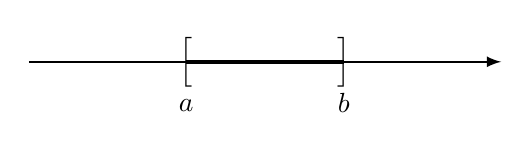
\begin{tikzpicture}[>=latex]
    \draw[thick,->] (0,0) --(6,0);
    \node[] at (2,0) {$\textbf{\Big[}$};
    \node[] at (4,0) {$\Big]$};
    \node[below=10pt] at (2,0) {$a$};
    \node[below=8pt] at (4,0) {$b$};
    \draw[ultra thick,-] (2,0) --(4,0);
\end{tikzpicture} \vspace{-2mm} \\ \hline 
\large{$\left] a;b \right]$} & \large{$a < x \leq b$} & 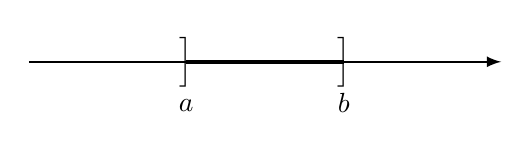
\begin{tikzpicture}[>=latex]
    \draw[thick,->] (0,0) --(6,0);
    \node[] at (2,0) {$\textbf{\Big]}$};
    \node[] at (4,0) {$\Big]$};
    \node[below=10pt] at (2,0) {$a$};
    \node[below=8pt] at (4,0) {$b$};
    \draw[ultra thick,-] (2,0) --(4,0);
\end{tikzpicture} \vspace{-2mm} \\ \hline 
\large{$\left[ a;b \right[$} & \large{$a \leq x < b$} & 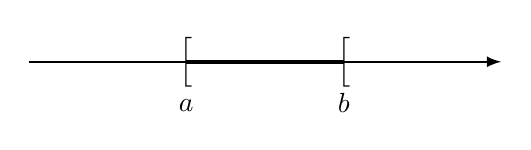
\begin{tikzpicture}[>=latex]
    \draw[thick,->] (0,0) --(6,0);
    \node[] at (2,0) {$\textbf{\Big[}$};
    \node[] at (4,0) {$\Big[$};
    \node[below=10pt] at (2,0) {$a$};
    \node[below=8pt] at (4,0) {$b$};
    \draw[ultra thick,-] (2,0) --(4,0);
\end{tikzpicture} \vspace{-2mm} \\ \hline 
\large{$\left] a;b \right[$} & \large{$a < x < b$} & 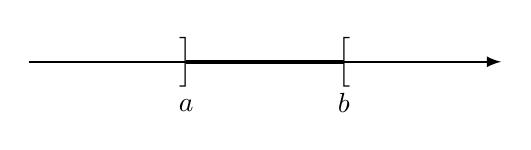
\begin{tikzpicture}[>=latex]
    \draw[thick,->] (0,0) --(6,0);
    \node[] at (2,0) {$\textbf{\Big]}$};
    \node[] at (4,0) {$\Big[$};
    \node[below=10pt] at (2,0) {$a$};
    \node[below=8pt] at (4,0) {$b$};
    \draw[ultra thick,-] (2,0) --(4,0);
\end{tikzpicture} \vspace{-2mm} \\ \hline 
\large{$\left] - \infty;b \right]$} & \large{$x \leq b$} & 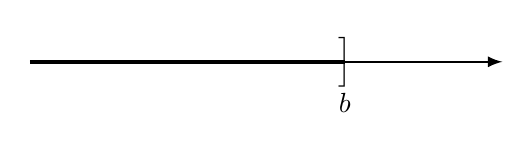
\begin{tikzpicture}[>=latex]
    \draw[thick,->] (0,0) --(6,0);
    \node[] at (4,0) {$\Big]$};
    \node[below=8pt] at (4,0) {$b$};
    \draw[ultra thick,-] (0,0) --(4,0);
\end{tikzpicture} \vspace{-2mm} \\ \hline 
\large{$\left] - \infty;b \right[$} & \large{$x < b$} & 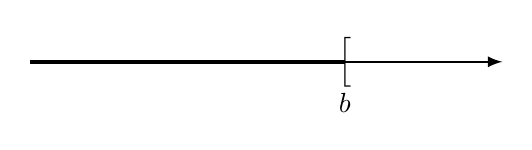
\begin{tikzpicture}[>=latex]
    \draw[thick,->] (0,0) --(6,0);
    \node[] at (4,0) {$\Big[$};
    \node[below=8pt] at (4,0) {$b$};
    \draw[ultra thick,-] (0,0) --(4,0);
\end{tikzpicture} \vspace{-2mm} \\ \hline 
\large{$\left[ a;+ \infty \right[$} & \large{$a \leq x $} & 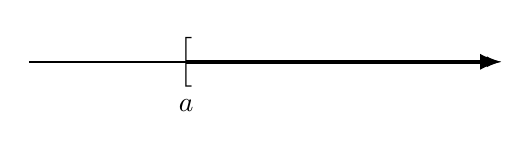
\begin{tikzpicture}[>=latex]
    \draw[thick,->] (0,0) --(6,0);
    \node[] at (2,0) {$\textbf{\Big[}$};
    \node[below=10pt] at (2,0) {$a$};
    \draw[ultra thick,->] (2,0) --(6,0);
\end{tikzpicture} \vspace{-2mm} \\ \hline 
\large{$\left] a; + \infty \right[$} & \large{$a < x$} & 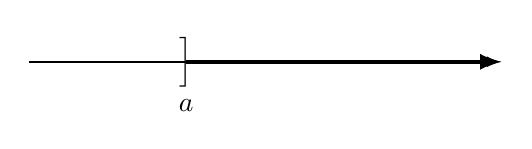
\begin{tikzpicture}[>=latex]
    \draw[thick,->] (0,0) --(6,0);
    \node[] at (2,0) {$\textbf{\Big]}$};
    \node[below=10pt] at (2,0) {$a$};
    \draw[ultra thick,->] (2,0) --(6,0);
\end{tikzpicture} \vspace{-2mm} \\ \hline
\end{tabularx}
\end{center}

\vspace{2cm}

\begin{center}
\begin{tabularx}{\textwidth}{ 
  | >{\centering\arraybackslash}c 
  | >{\centering\arraybackslash}X
  | >{\centering\arraybackslash}X | }
\hline
L'intervalle noté $\ldots$ & $\ldots$ désigne l'ensemble des réels $x$ tels que $\ldots$ & Il est représenté par un segment sur une droite graduée\\ \hline 
\large{$\left[ a;b \right]$} & \large{$a \leq x \leq b$} & 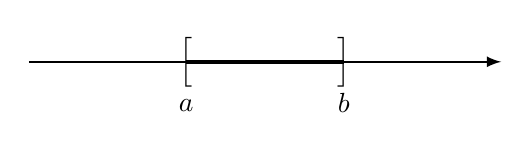
\begin{tikzpicture}[>=latex]
    \draw[thick,->] (0,0) --(6,0);
    \node[] at (2,0) {$\textbf{\Big[}$};
    \node[] at (4,0) {$\Big]$};
    \node[below=10pt] at (2,0) {$a$};
    \node[below=8pt] at (4,0) {$b$};
    \draw[ultra thick,-] (2,0) --(4,0);
\end{tikzpicture} \vspace{-2mm} \\ \hline 
\large{$\left] a;b \right]$} & \large{$a < x \leq b$} & 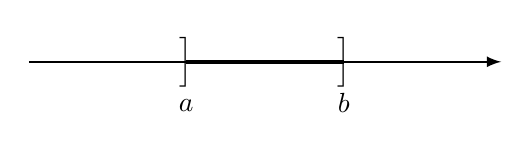
\begin{tikzpicture}[>=latex]
    \draw[thick,->] (0,0) --(6,0);
    \node[] at (2,0) {$\textbf{\Big]}$};
    \node[] at (4,0) {$\Big]$};
    \node[below=10pt] at (2,0) {$a$};
    \node[below=8pt] at (4,0) {$b$};
    \draw[ultra thick,-] (2,0) --(4,0);
\end{tikzpicture} \vspace{-2mm} \\ \hline 
\large{$\left[ a;b \right[$} & \large{$a \leq x < b$} & 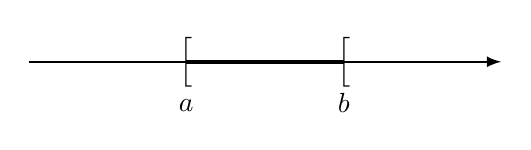
\begin{tikzpicture}[>=latex]
    \draw[thick,->] (0,0) --(6,0);
    \node[] at (2,0) {$\textbf{\Big[}$};
    \node[] at (4,0) {$\Big[$};
    \node[below=10pt] at (2,0) {$a$};
    \node[below=8pt] at (4,0) {$b$};
    \draw[ultra thick,-] (2,0) --(4,0);
\end{tikzpicture} \vspace{-2mm} \\ \hline 
\large{$\left] a;b \right[$} & \large{$a < x < b$} & 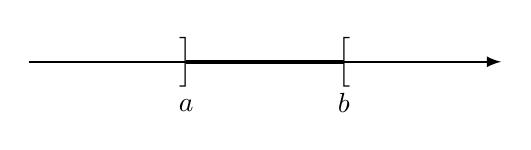
\begin{tikzpicture}[>=latex]
    \draw[thick,->] (0,0) --(6,0);
    \node[] at (2,0) {$\textbf{\Big]}$};
    \node[] at (4,0) {$\Big[$};
    \node[below=10pt] at (2,0) {$a$};
    \node[below=8pt] at (4,0) {$b$};
    \draw[ultra thick,-] (2,0) --(4,0);
\end{tikzpicture} \vspace{-2mm} \\ \hline 
\large{$\left] - \infty;b \right]$} & \large{$x \leq b$} & 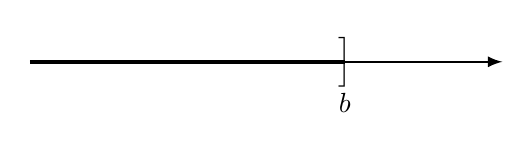
\begin{tikzpicture}[>=latex]
    \draw[thick,->] (0,0) --(6,0);
    \node[] at (4,0) {$\Big]$};
    \node[below=8pt] at (4,0) {$b$};
    \draw[ultra thick,-] (0,0) --(4,0);
\end{tikzpicture} \vspace{-2mm} \\ \hline 
\large{$\left] - \infty;b \right[$} & \large{$x < b$} & 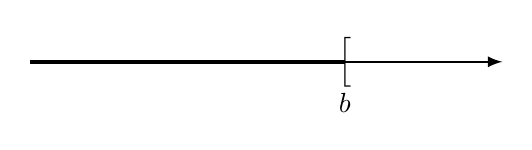
\begin{tikzpicture}[>=latex]
    \draw[thick,->] (0,0) --(6,0);
    \node[] at (4,0) {$\Big[$};
    \node[below=8pt] at (4,0) {$b$};
    \draw[ultra thick,-] (0,0) --(4,0);
\end{tikzpicture} \vspace{-2mm} \\ \hline 
\large{$\left[ a;+ \infty \right[$} & \large{$a \leq x $} & 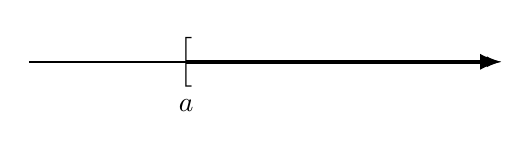
\begin{tikzpicture}[>=latex]
    \draw[thick,->] (0,0) --(6,0);
    \node[] at (2,0) {$\textbf{\Big[}$};
    \node[below=10pt] at (2,0) {$a$};
    \draw[ultra thick,->] (2,0) --(6,0);
\end{tikzpicture} \vspace{-2mm} \\ \hline 
\large{$\left] a; + \infty \right[$} & \large{$a < x$} & 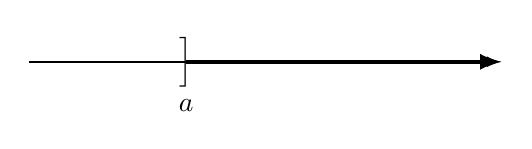
\begin{tikzpicture}[>=latex]
    \draw[thick,->] (0,0) --(6,0);
    \node[] at (2,0) {$\textbf{\Big]}$};
    \node[below=10pt] at (2,0) {$a$};
    \draw[ultra thick,->] (2,0) --(6,0);
\end{tikzpicture} \vspace{-2mm} \\ \hline
\end{tabularx}
\end{center}

\end{document}